\newcommand{\department}{САПР}
\newcommand{\lablabel}{КУРСОВАЯ РАБОТА}
\newcommand{\hasnum}{0}
\newcommand{\labnum}{1}
\newcommand{\discipline}{Алгоритмы и структуры данных}
\newcommand{\theme}{Преобразование алгебраических формул из инфиксной в постфиксную форму записи и вычисление значения выражения(вариант 1)}
\newcommand{\haspartner}{0}
\newcommand{\partnername}{None}
\newcommand{\teachername}{Тутуева А.В.}
\newcommand{\labyear}{2021}

%%%%%%%%%%%%%%%%%%%%% General stuff %%%%%%%%%%%%%%%%%%%%%%%%%%%

\documentclass[12pt,a4paper]{article}  % шаблон для статьи, шрифт 12 пт

\usepackage[warn]{mathtext} % для отображения кириллицы в формулах (НУЖНО загружать ДО fontenc и babel)

\usepackage[utf8]{inputenc}  % использование кодировки Юникод UTF-8
\usepackage[T1]{fontenc}
\usepackage[russian]{babel}  % пакет поддержки русского языка

\usepackage{indentfirst}  % отступ первого абзаца
\setlength{\parindent}{0.75cm}

\usepackage[compact]{titlesec}  % для titlespacing
% \titlespacing{\заголовок}{слева}{перед}{после}[справа]
\titlespacing*{\section}{0.75cm}{1em}{0.1em}  % отступ заголовка
\titlespacing*{\subsection}{0.75cm}{1em}{0.1em}

%%%%%%%%%%%%%%%%%%%%% Pictures %%%%%%%%%%%%%%%%%%%%%%%%%%%

\usepackage{graphicx}  % кртинки
\usepackage{float} % плавающие картинки
\usepackage{wrapfig}  % Обтекание фигур (таблиц, картинок и прочего)
\usepackage[labelsep=endash]{caption}  % тире вместо двоеточия в картинках
\usepackage{subcaption} % place more than 1 figure at a picture

%%%%%%%%%%%%%%%%%%%%% Math symbols %%%%%%%%%%%%%%%%%%%%%%%%%%%

% \DeclareSymbolFont{T2Aletters}{T2A}{cmr}{m}{it} % переопределение шрифта для кириллицы в формулах на курсив
\usepackage{amsmath}

%%%%%%%%%%%%%%%%%%%%% Code %%%%%%%%%%%%%%%%%%%%%%%%%%%

\usepackage{xcolor}
\usepackage{listings}  % листинги кода из файлов

\definecolor{codegreen}{rgb}{0,0.6,0}
\definecolor{codegray}{rgb}{0.5,0.5,0.5}
\definecolor{codepurple}{rgb}{0.58,0,0.82}
\definecolor{backcolour}{rgb}{0.95,0.95,0.92}

\lstdefinestyle{cpp}
{
    backgroundcolor=\color{backcolour},% цвет фона подсветки
    commentstyle=\color{codegreen},
    keywordstyle=\color{magenta},
    numberstyle=\small\color{codegray},% размер шрифта для номеров строк
    stringstyle=\color{codepurple},
    basicstyle=\ttfamily\footnotesize, % размер и начертание шрифта для подсветки кода
    breakatwhitespace=false,           % переносить строки только если есть пробел  
    breaklines=true,                   % автоматически переносить строки (да\нет)  
    captionpos=t,                      % позиция заголовка вверху [t] или внизу [b]
    keepspaces=true,                 
    numbers=left,                   % где поставить нумерацию строк (слева\справа)            
    numbersep=5pt,                  % как далеко отстоят номера строк от подсвечиваемого кода           
    showspaces=false,               % показывать или нет пробелы специальными отступами       
    showstringspaces=false,         % показывать или нет пробелы в строках
    showtabs=false,                 % показывать или нет табуляцию в строках        
    tabsize=2,                      % размер табуляции по умолчанию равен 2 пробелам
    language=c++,                   % выбор языка для подсветки (здесь это С++)                   
    stepnumber=1,                   % размер шага между двумя номерами строк
    frame=false,                    % рисовать рамку вокруг кода
    escapeinside={\%*}{*)},         % если нужно добавить комментарии в коде
    extendedchars=\true
}

\lstdefinelanguage
[x64]{Assembler}     % add a "x64" dialect of Assembler
[x86masm]{Assembler} % based on the "x86masm" dialect
% with these extra keywords:
{morekeywords={PUSH, POP, LDI, SBI, CBI}} % etc.

\lstdefinestyle{myasm}
{
    backgroundcolor=\color{backcolour},% цвет фона подсветки
    commentstyle=\color{codegreen},
    keywordstyle=\color{magenta},
    numberstyle=\small\color{codegray},% размер шрифта для номеров строк
    stringstyle=\color{codepurple},
    basicstyle=\ttfamily\footnotesize, % размер и начертание шрифта для подсветки кода
    breakatwhitespace=false,           % переносить строки только если есть пробел  
    breaklines=true,                   % автоматически переносить строки (да\нет)  
    captionpos=t,                      % позиция заголовка вверху [t] или внизу [b]
    keepspaces=true,                 
    numbers=left,                   % где поставить нумерацию строк (слева\справа)            
    numbersep=5pt,                  % как далеко отстоят номера строк от подсвечиваемого кода           
    showspaces=false,               % показывать или нет пробелы специальными отступами       
    showstringspaces=false,         % показывать или нет пробелы в строках
    showtabs=false,                 % показывать или нет табуляцию в строках        
    tabsize=2,                      % размер табуляции по умолчанию равен 2 пробелам
    language=[x64]Assembler,             % выбор языка для подсветки             
    stepnumber=1,                   % размер шага между двумя номерами строк
    frame=false,                    % рисовать рамку вокруг кода
    escapeinside={\%*}{*)},         % если нужно добавить комментарии в коде
    extendedchars=\true
}

\lstset{style=myasm}

%%%%%%%%%%%%%%%%%%%%% Other %%%%%%%%%%%%%%%%%%%%%%%%%%%

\usepackage{comment}

%\usepackage[showframe=true]{geometry} % shows the borders of the pages content
\usepackage{changepage} % Для смещения таблиц влево

\begin{document}

    \thispagestyle{empty}

\begin{center}
    \Large{
	    \textbf{МИНОБРНАУКИ РОССИИ}
	
	    \textbf{Санкт-Петербургский государственный}
	
	    \textbf{электротехнический университет «ЛЭТИ»}
	
	    \textbf{им. В.И. Ульянова (Ленина)}
	
	    \textbf{Кафедра \department}
    }
\end{center}

\topskip=0pt
\vspace*{\fill}

\begin{center}
    \Large{
	    \textbf{
		    \lablabel 
		        \if \hasnum 1 
		        №\labnum 
		        \fi
		        \\
		    по дисциплине «\discipline»\\
		    Тема: \theme\\
	    }
    }
\end{center}

\vspace*{\fill}

\begin{tabular}{lcr}
    Студент\if \haspartner 1ы \fi\ гр. 9892 & \begin{tabular}{p{60mm}} \\ \hline \end{tabular} & Лескин К.А.  \\\\
    \if \haspartner 1
                      & \begin{tabular}{p{60mm}} \\ \hline \end{tabular} & \partnername \\\\
    \fi
    Преподаватель     & \begin{tabular}{p{60mm}} \\ \hline \end{tabular} & \teachername
    \\\\
\end{tabular}

\begin{center}
    Санкт-Петербург\\
    \labyear
\end{center}

\newpage

    
    \section*{Задача}

Необходимо реализовать простейшую версию калькулятора.
Пользователю должен быть доступен ввод математического выражения,
состоящего из чисел и арифметических знаков.

Программа должна выполнить проверку корректности введенного выражения.
В случае некорректного ввода необходимо вывести сообщение об ошибке
с указанием позиции некорректного ввода.
В противном выводится обратная польская нотация введенного
выражения, а также отображается результат вычисления.

Входные данные:

\begin{itemize}
    \item арифметическое выражение
    \item поддерживаемый тип данных: вещественные числа (double)
    \item поддерживаемые знаки: $ +, -, *, /, ^, $ унарный $ - $, функции с одним
    аргументом ($ cos, sin, tg, ctg, ln, log, sqrt $ и др. (хотя бы одну не из списка)),
    \item константы pi, e открывающая и закрывающая скобки
\end{itemize}

Выходные данные:

\begin{itemize}
    \item постфиксная ФЗ
    \item результат вычисления
\end{itemize}

Входные данные по желанию можно читать из файла.

    \section*{Обоснование выбора используемых структур данных}

Каждая нотация состоит из токенов типа \verb|Token|.
Конкретные типы токенов, будь то константа, операнд или функция,
наследуются от \verb|Token|.

Для строго ограниченных токенов
(операторы, функции, скобки, константы)
определены группы токенов и с их определениями.
Создание токенов из групп происходит
посредством вызова метода группы токенов.
Это необходимо для того, чтобы абстрагировать
создание токенов с особыми параметрами,
такими как приоритет операции,
ассоциативность (унарность),
коллбэк для операторов,
значение констант и т.д.

Определение (наследник класса \verb|Definition|)
содержит основные параметры для создания новых токенов из групп.

Для нотаций были реализованы три класса:

\verb|InfixExpression|,

\verb|PrefixExpression|,

\verb|PostfixExpression|.

Все классы для нотаций реализуют методы валидации и
вычисления конкретной нотации.
Общее для всех нотаций поведение содержится в базовом классе
\verb|BaseExpression|, включающее в себя
токенизацию строки с выражением с помощью класса \verb|Tokenizer|,
получение выражение в виде строки
и пр.

Для конвертации выражения одной нотации в другую
используется класс \verb|Converter|.



    \section*{Описание алгоритма решения}

Работа выполнена в виде библиотеки \verb|expressions|
и главного файла \verb|main.py|, использующего
библиотеку.

\subsection*{Главный скрипт main.py}

\verb|main.py| представляет собой бесконечный цикл
ввода выражений.
Цикл заканчивается, если введена пустая строка.
Перед каждым вводом об этом сообщается пользователю,
как и список доступных математических функций.

Нотация, в которой введено выражение, автоматически определяется
с помощью функции \verb|get_expression(expression)|,
которая пытается создать из введённой строки объект выражения и венуть его.
Если создание не получилось, возвращается \verb|None|,
а цикл начинается заново.

Если в выражении есть переменные,
пользователю предлагается ввести значение каждой из них.
Ввод обрабатывается на наличие ошибок.
После ввода в выражение подставляются значения переменных.

Далее введённое выражение конвертируется во все нотации.
На экран выводятся строковые репрезентации всех выражений,
а так же их вычисленные значения.
После этого цикл начинается сначала.

\subsection*{Нотации}

Создание нотации включает шаги:

\begin{enumerate}
    \item Токенизировать входную строку
    \item Провалидировать список токенов
        \subitem Задать значения переменных по умолчанию
        \subitem Выполнить предварительную валидацию (проверка corner cases).
        \subitem Попытаться вычислить выражение.
\end{enumerate}

\subsection*{Конвертация}

Так как нотаций три, возможны 6 видов конвертаций.
Для упрощения выполнения задачи были реализованы три алгоритма,
связывающих нотации "треугольником":
инфиксная в постфиксную,
постфиксная в префиксную,
префиксная в инфиксную.
Это позволяет конвертировать нотации "из любой в любую".
Например, для конвертации из инфиксной в префиксную,
нужно сначала конвертировать инфиксную в постфиксную,
а затем постфиксную в префиксную.

    \section*{Пример работы}

На рисунке \ref{fig:example} прдставлен пример выпонения программы

\begin{figure}[H]
    \centering
    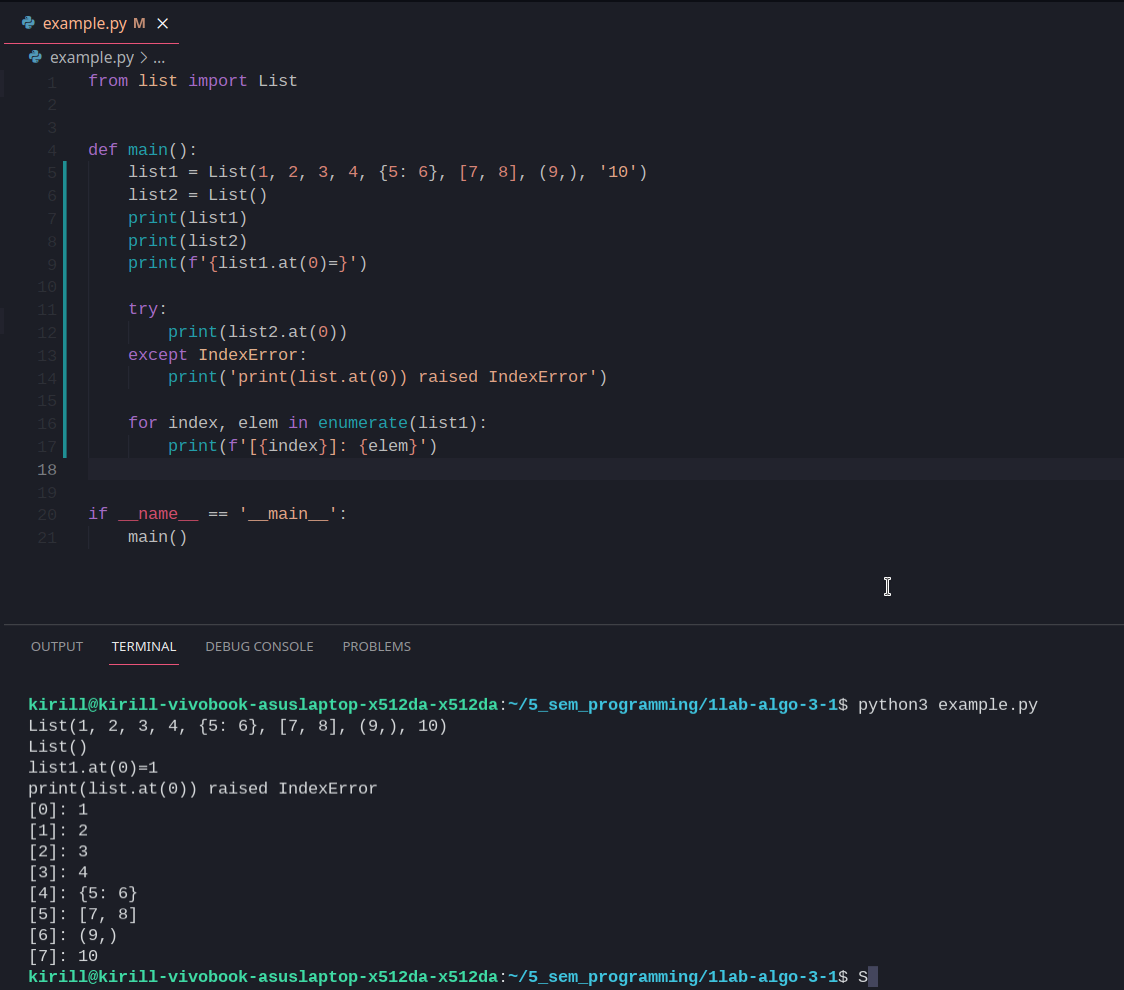
\includegraphics[width=\linewidth]{photo/example}
    \caption{Пример выполнения демонстрационной программы}
    \label{fig:example}
\end{figure}

    \section*{Листинг}

Исходный код программы доступен по ссылке: 

https://github.com/kira607/cw-algo-3-1

\end{document}
